% ============================================================================
% LiteForge -- PowerShell / VDI Install and Quickstart Guide
% LiteForge
% ============================================================================
\documentclass[11pt,letterpaper]{article}

% --- Packages ---
\usepackage[T1]{fontenc}
\usepackage[utf8]{inputenc}
\usepackage[margin=1in]{geometry}
\usepackage{fancyhdr}
\usepackage[dvipsnames,table]{xcolor}
\usepackage{booktabs}
\usepackage{listings}
\usepackage[colorlinks=true]{hyperref}
\usepackage{tikz}
\usepackage[most]{tcolorbox}
\usepackage{tabularx}
\usepackage{enumitem}
\usepackage{parskip}
\usepackage{lmodern}
\usepackage{helvet}
\renewcommand{\familydefault}{\sfdefault}
\usepackage{graphicx}
\usepackage{titlesec}
\usepackage{setspace}
\usepackage{float}
\usepackage[font=small,labelfont=bf]{caption}

\usetikzlibrary{
  arrows.meta,positioning,shapes.geometric,fit,backgrounds,calc,
  decorations.pathreplacing,shapes.multipart,chains,matrix
}

% ---- Walter palette (light background) ----
\definecolor{navybg}{HTML}{0E2841}
\definecolor{navylight}{HTML}{152F4A}
\definecolor{walterpurple}{HTML}{715ABF}
\definecolor{walterorange}{HTML}{F08940}
\definecolor{walterdarkpurple}{HTML}{503F86}
\definecolor{copper}{HTML}{B86B4A}
\definecolor{recgreen}{HTML}{5AAF42}
\definecolor{alertred}{HTML}{B71C1C}
\definecolor{tipblue}{HTML}{2A7AB5}
\definecolor{tipgreen}{HTML}{5AAF42}
\definecolor{tiporange}{HTML}{F08940}
\definecolor{tipred}{HTML}{DC2626}
\definecolor{forgegray}{HTML}{666666}
\definecolor{lightgray}{HTML}{F5F5F5}
\definecolor{bordergray}{HTML}{DDDDDD}
\definecolor{codebg}{HTML}{F5F5F5}
\definecolor{codeframe}{HTML}{DDDDDD}

% --- Light page (white bg, navy text) ---
\color{navybg}
\arrayrulecolor{bordergray}
\hypersetup{linkcolor=tipblue, urlcolor=tipblue, citecolor=tipblue}

% --- Section heading colors ---
\titleformat{\section}
  {\Large\bfseries\color{navybg}}{\thesection}{1em}{}
\titleformat{\subsection}
  {\large\bfseries\color{walterpurple}}{\thesubsection}{1em}{}
\titleformat{\subsubsection}
  {\normalsize\bfseries\color{tipblue}}{\thesubsubsection}{1em}{}

% --- tcolorbox styles ---
\tcbset{
  tipbox/.style={
    enhanced, colback=tipgreen!5, colframe=tipgreen!50,
    colbacktitle=tipgreen!80, coltitle=white, coltext=navybg,
    fonttitle=\bfseries, title=#1,
    boxrule=0.5pt, arc=2pt, toptitle=4pt, bottomtitle=4pt,
    left=8pt, right=8pt, top=6pt, bottom=6pt,
  },
  warnbox/.style={
    enhanced, colback=alertred!5, colframe=alertred!50,
    colbacktitle=alertred!80, coltitle=white, coltext=navybg,
    fonttitle=\bfseries, title=#1,
    boxrule=0.5pt, arc=2pt, toptitle=4pt, bottomtitle=4pt,
    left=8pt, right=8pt, top=6pt, bottom=6pt,
  },
  infobox/.style={
    enhanced, colback=tipblue!5, colframe=tipblue!50,
    colbacktitle=tipblue!80, coltitle=white, coltext=navybg,
    fonttitle=\bfseries, title=#1,
    boxrule=0.5pt, arc=2pt, toptitle=4pt, bottomtitle=4pt,
    left=8pt, right=8pt, top=6pt, bottom=6pt,
  },
  notebox/.style={
    enhanced, colback=walterpurple!5, colframe=walterpurple!40,
    colbacktitle=walterpurple!80, coltitle=white, coltext=navybg,
    fonttitle=\bfseries, title=#1,
    boxrule=0.5pt, arc=2pt, toptitle=4pt, bottomtitle=4pt,
    left=8pt, right=8pt, top=6pt, bottom=6pt,
  },
  stepbox/.style={
    enhanced, colback=walterorange!5, colframe=walterorange!50,
    colbacktitle=walterorange!80, coltitle=white, coltext=navybg,
    fonttitle=\bfseries, title=#1,
    boxrule=0.5pt, arc=2pt, toptitle=4pt, bottomtitle=4pt,
    left=8pt, right=8pt, top=6pt, bottom=6pt,
  },
}

% --- Listings ---
\lstset{
  basicstyle=\ttfamily\small\color{navybg},
  backgroundcolor=\color{codebg},
  frame=single,
  rulecolor=\color{codeframe},
  breaklines=true,
  breakatwhitespace=false,
  breakautoindent=true,
  columns=fullflexible,
  keepspaces=true,
  showstringspaces=false,
  tabsize=2,
  xleftmargin=4pt,
  xrightmargin=4pt,
  aboveskip=8pt,
  belowskip=8pt,
}

\lstdefinestyle{powershell}{
  language={},
  keywordstyle=\color{tipblue}\bfseries,
  stringstyle=\color{tipgreen},
  commentstyle=\color{forgegray}\itshape,
  morekeywords={Invoke-WebRequest,Remove-Item,Get-Command,Set-ExecutionPolicy,Start-Sleep,git,clone,cargo,python,pip,forge,winget},
}

\lstdefinestyle{bash}{
  language=bash,
  keywordstyle=\color{tipblue}\bfseries,
  stringstyle=\color{tipgreen},
  commentstyle=\color{forgegray}\itshape,
  morekeywords={forge,claude},
}

% --- Header / Footer ---
\pagestyle{fancy}
\fancyhf{}
\fancyhead[L]{\small\color{forgegray}LiteForge -- PowerShell / VDI Install Guide}
\fancyhead[R]{\small\color{forgegray}LiteForge}
\fancyfoot[C]{\small\color{forgegray}\thepage}
\fancyfoot[R]{\tiny\color{alertred}\textit{Proprietary and Confidential}}
\renewcommand{\headrulewidth}{0.4pt}
\renewcommand{\footrulewidth}{0.2pt}

% --- Graphics path ---
\graphicspath{{images/}}

% ============================================================================
\begin{document}

% ---- Title Page ----
\begin{titlepage}
\centering
\vspace*{2cm}

{\Huge\bfseries\color{navybg}LiteForge}\\[6pt]
{\Large\color{walterpurple}PowerShell / VDI Install and Quickstart Guide}

\vspace{1.5cm}


\begin{tikzpicture}
  \draw[walterorange, line width=2pt] (0,0) -- (10,0);
\end{tikzpicture}

\vspace{1.5cm}

{\large Sean Poyner}\\[4pt]
{\normalsize\color{forgegray}Senior Director, AI Engineering (Use Case)}\\[4pt]
{\normalsize\color{forgegray}Data, AI \& Emerging Technology Guild}\\[12pt]
{\normalsize LiteForge}

\vspace{1.5cm}

{\normalsize May 2026}

\vfill

{\small\color{alertred}\textbf{LiteForge}}
\end{titlepage}

% ---- Table of Contents ----
\tableofcontents
\newpage

% ============================================================================
\section{Overview}
% ============================================================================

The \textbf{Travel Innovation Platform (LiteForge) SDK} provides a CLI tool
(\texttt{forge}), Python and Rust SDKs, and an Agent Development Kit for
building AI-powered applications on internal LLM gateway.

This guide walks through installing LiteForge on a \textbf{Windows VDI}
using \textbf{native Windows PowerShell} (no WSL required). It covers the
prerequisites unique to a VDI environment --- Rust, the Visual C++ Build
Tools with the Windows SDK, Python, and (optionally) Node.js --- plus the
steps to clone and run the installer. By the end you will have a working
\texttt{forge} CLI and any combination of the Python, Node.js, and Rust SDKs
that match the toolchains you have installed.

\begin{tcolorbox}[infobox={Prerequisites}]
\textbf{Hardware / OS}
\begin{itemize}[nosep]
  \item Windows 10/11 (64-bit), VDI or local
  \item PowerShell 5.1 or later (ships with Windows)
  \item $\sim$8\,GB free disk (Visual C++ Build Tools alone is $\sim$2\,GB,
    plus Rust toolchain, build artifacts, and crate cache)
  \item Internet access to \texttt{gitea.poyner.ai},
    \texttt{aka.ms} / \texttt{visualstudio.com}, \texttt{win.rustup.rs},
    \texttt{python.org}, and \texttt{nodejs.org}
\end{itemize}
\textbf{Accounts \& credentials}
\begin{itemize}[nosep]
  \item GitHub Enterprise credentials (\texttt{gitea.poyner.ai})
  \item LiteForge API key (obtain from your team lead or the LiteForge.ai portal ---
    starts with \texttt{sk-z-})
\end{itemize}
\textbf{Tools you will install in this guide} (each step covers one)
\begin{itemize}[nosep]
  \item \textbf{Step 1:} Rust toolchain (\texttt{rustup}, \texttt{cargo})
  \item \textbf{Step 2:} Visual C++ Build Tools \emph{including the
    Windows 10 or 11 SDK} (provides \texttt{link.exe} and
    \texttt{kernel32.lib})
  \item \textbf{Step 3:} Python 3.12 (recommended; matches the bundled
    pre-built wheel)
  \item \textbf{Step 4 (optional):} Node.js LTS for \texttt{liteforge-js}
\end{itemize}
\textbf{Permissions}
\begin{itemize}[nosep]
  \item Local install rights for the user (no admin required for Rust,
    Python user-install, or the bundled binaries; admin is required for
    the Visual C++ Build Tools installer)
  \item Ability to add user-level environment variables (the installer
    writes \texttt{LiteForge\_API\_KEY}, \texttt{LiteForge\_BASE\_URL}, etc. to
    HKCU)
\end{itemize}
\end{tcolorbox}

\begin{tcolorbox}[notebox={Why not WSL?}]
WSL is the recommended path when available. This guide is for VDI sessions
where WSL is not enabled, not allowed, or not desired. The installer ships
a pre-built Windows binary inside the repository, so you do \emph{not} need
to compile anything locally if the network blocks the GitHub release
download.
\end{tcolorbox}

\newpage
% ============================================================================
\section{Step 1: Install Rust}
% ============================================================================

Rust is required by the installer to build the Python SDK from source.
Even though the CLI ships as a pre-built binary, \texttt{cargo} must be on
the PATH for the installer to satisfy the Python wheel build path on Python
versions that don't match the bundled wheel.

Open a new \textbf{Windows PowerShell} window and run:

\begin{lstlisting}[style=powershell]
Invoke-WebRequest -Uri https://win.rustup.rs/x86_64 -OutFile $env:TEMP\rustup-init.exe
& $env:TEMP\rustup-init.exe -y
Remove-Item $env:TEMP\rustup-init.exe
\end{lstlisting}

\begin{figure}[H]
\centering
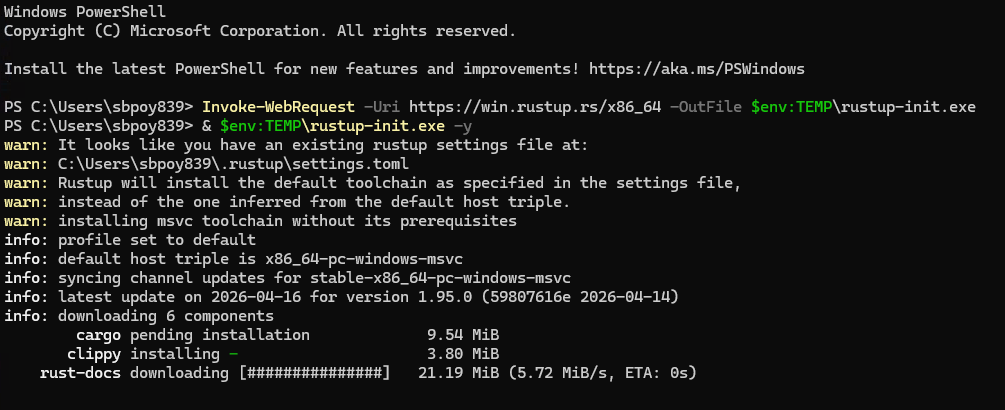
\includegraphics[width=0.95\textwidth]{ps-vdi-01-rustup-install.png}
\caption{\texttt{rustup-init.exe -y} downloads the default
\texttt{x86\_64-pc-windows-msvc} toolchain non-interactively.}
\end{figure}

After installation completes, reload PATH and verify:

\begin{lstlisting}[style=powershell]
$env:Path = [System.Environment]::GetEnvironmentVariable("Path","User") + ";" + [System.Environment]::GetEnvironmentVariable("Path","Machine")
cargo --version
\end{lstlisting}

\begin{figure}[H]
\centering
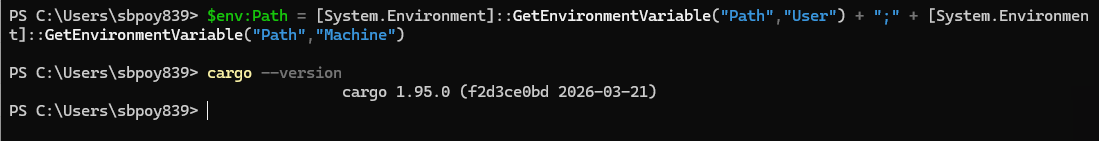
\includegraphics[width=0.95\textwidth]{ps-vdi-02-cargo-verify.png}
\caption{\texttt{cargo --version} reports a successful install.}
\end{figure}

\begin{tcolorbox}[warnbox={Don't skip the PATH reload}]
The installer writes \texttt{cargo} to \texttt{\%USERPROFILE\%\textbackslash.cargo\textbackslash bin}
and updates the \emph{user} PATH, but PowerShell only reads PATH on launch.
Either run the \texttt{\$env:Path = ...} line above or close and re-open
PowerShell before continuing.
\end{tcolorbox}

\newpage
% ============================================================================
\section{Step 2: Install Visual C++ Build Tools}
% ============================================================================

Rust on Windows uses the \textbf{MSVC} linker (\texttt{link.exe}) and the
\textbf{Windows SDK} (\texttt{kernel32.lib}). The Build Tools installer is
the smallest way to satisfy both. We recommend the \textbf{interactive GUI
install} on a VDI --- silent installs frequently appear to succeed but skip
the SDK component.

Download and launch the Build Tools installer:

\begin{lstlisting}[style=powershell]
Invoke-WebRequest -Uri https://aka.ms/vs/17/release/vs_buildtools.exe -OutFile $env:TEMP\vs_buildtools.exe
& $env:TEMP\vs_buildtools.exe
\end{lstlisting}

\begin{figure}[H]
\centering
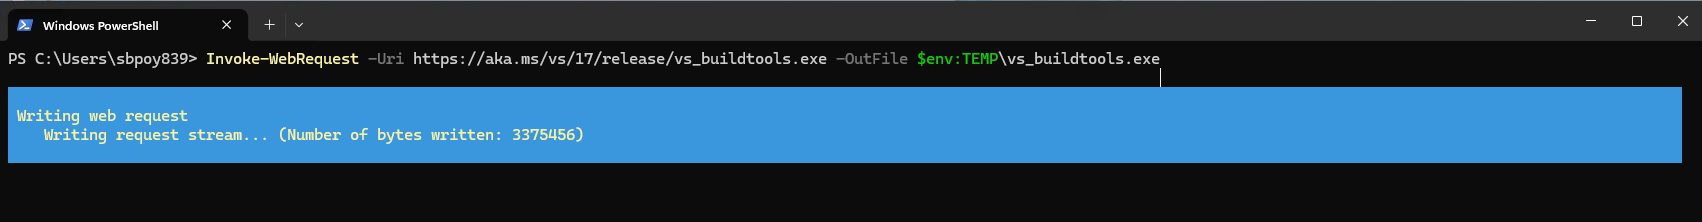
\includegraphics[width=0.95\textwidth]{ps-vdi-03-vs-download.png}
\caption{The Build Tools bootstrapper downloads (a few MB), then launches
the full installer.}
\end{figure}

\subsection{Approve the UAC prompt}

\begin{figure}[H]
\centering
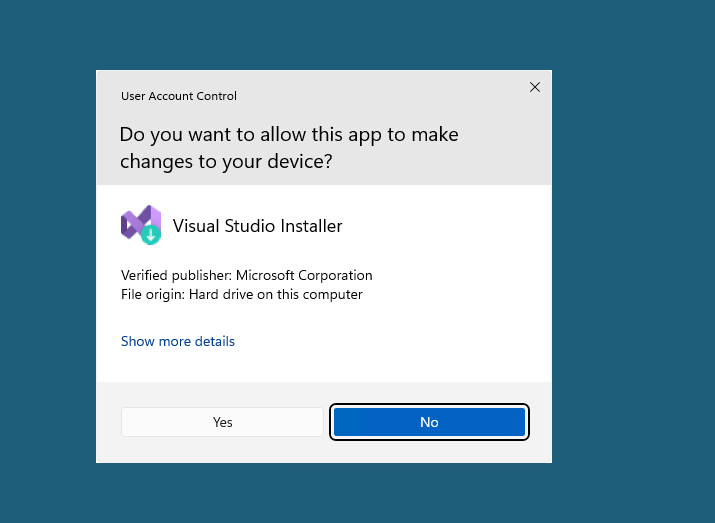
\includegraphics[width=0.55\textwidth]{ps-vdi-04-uac-prompt.png}
\caption{Windows asks if Visual Studio Installer can make changes ---
click \textbf{Yes}.}
\end{figure}

\begin{figure}[H]
\centering
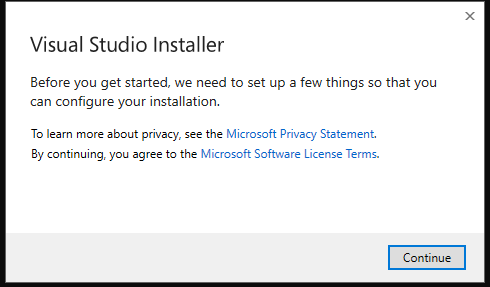
\includegraphics[width=0.55\textwidth]{ps-vdi-05-vs-welcome.png}
\caption{First-time setup screen. Click \textbf{Continue}.}
\end{figure}

\subsection{Modify or install the workload}

If Build Tools 2022 is already installed, click \textbf{Modify}. Otherwise
the installer opens directly to workload selection.

\begin{figure}[H]
\centering
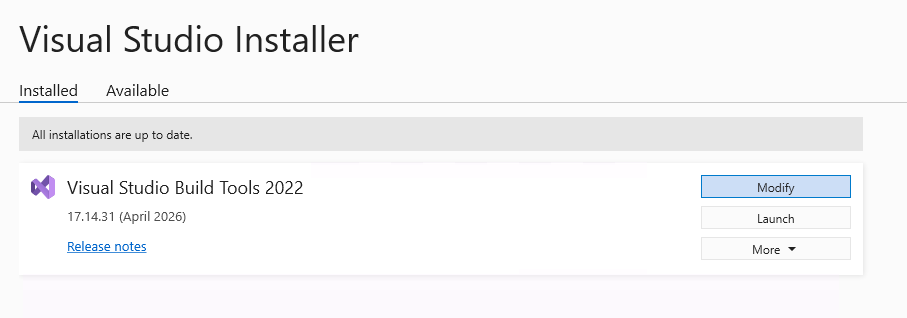
\includegraphics[width=0.95\textwidth]{ps-vdi-06-vs-modify.png}
\caption{Visual Studio Installer with Build Tools 2022 already present ---
click \textbf{Modify} to add components.}
\end{figure}

In the \textbf{Workloads} tab, check \textbf{Desktop development with
C++}. This selects the linker and the C++ build tools.

\begin{figure}[H]
\centering
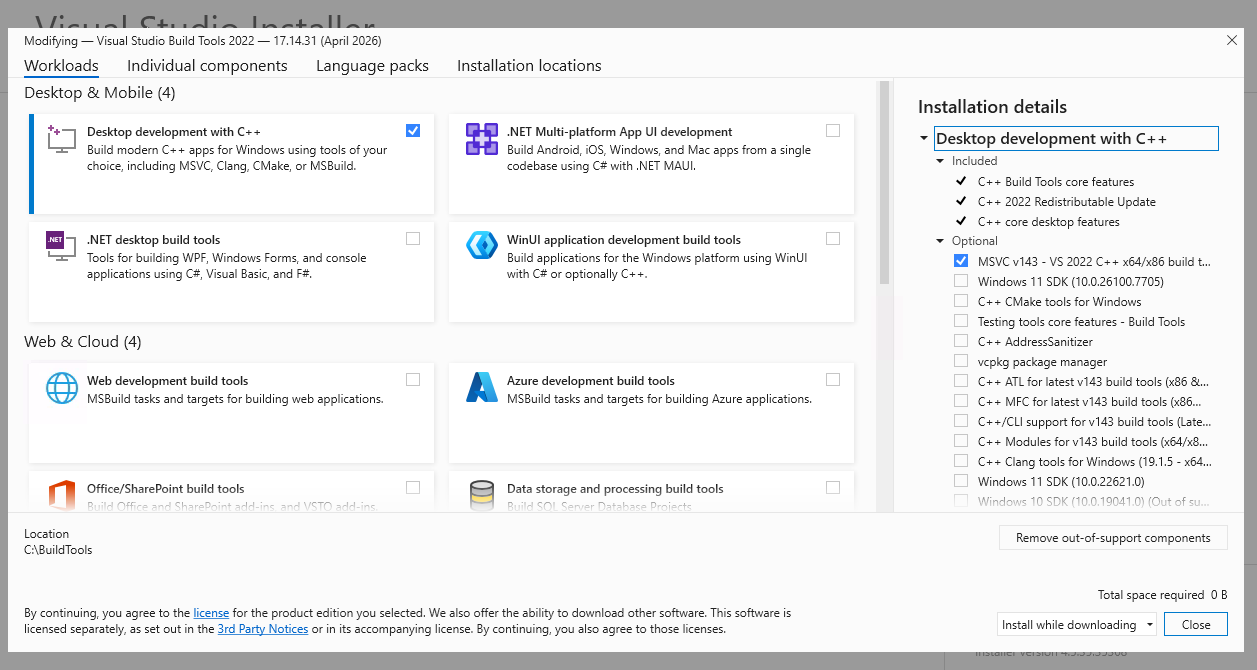
\includegraphics[width=0.95\textwidth]{ps-vdi-07-vs-workload.png}
\caption{Check \textbf{Desktop development with C++}. The right-hand
\textit{Installation details} panel lists what gets installed.}
\end{figure}

In the right-hand panel under \textbf{Optional}, ensure both
\textbf{MSVC v143 -- VS 2022 C++ x64/x86 build tools} and the most recent
\textbf{Windows 11 SDK} (or Windows 10 SDK) are checked, then click
\textbf{Modify} (or \textbf{Install}).

\begin{figure}[H]
\centering
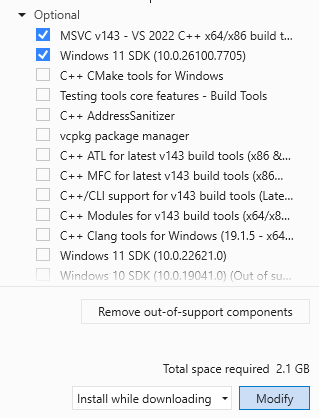
\includegraphics[width=0.55\textwidth]{ps-vdi-08-vs-components.png}
\caption{Required optional components: \textbf{MSVC v143} and a
\textbf{Windows SDK}. Total size is roughly 2.1\,GB.}
\end{figure}

\begin{tcolorbox}[warnbox={The Windows SDK is mandatory}]
Without the Windows SDK, the linker fails with:
\begin{lstlisting}[style=powershell]
LINK : fatal error LNK1181: cannot open input file 'kernel32.lib'
\end{lstlisting}
This is the most common reason \texttt{cargo build} fails on a
freshly-provisioned VDI. The MSVC compiler alone is not enough.
\end{tcolorbox}

\subsection{Wait for the install}

\begin{figure}[H]
\centering
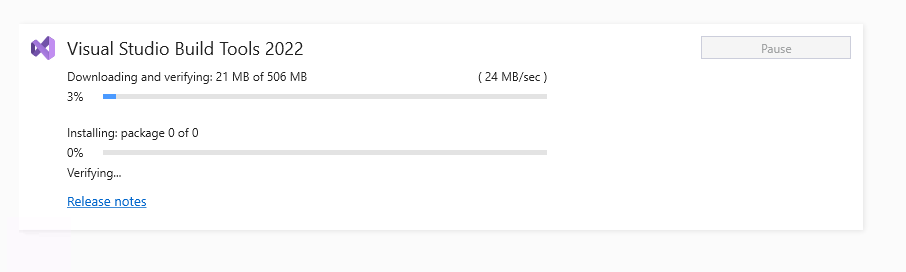
\includegraphics[width=0.95\textwidth]{ps-vdi-09-vs-installing.png}
\caption{The installer downloads and applies the workload ---
typically 10--15 minutes on VDI bandwidth.}
\end{figure}

When it finishes, \textbf{close and re-open PowerShell} so the new
environment variables (\texttt{INCLUDE}, \texttt{LIB}, etc.) are picked up.

\newpage
% ============================================================================
\section{Step 3: Install Python}
% ============================================================================

The installer uses Python 3.12 to install the \texttt{liteforge-py} wheel.
Earlier or later 3.x versions work, but the pre-built wheel shipped in the
repo is \texttt{cp312} and gives the cleanest path.

\subsection{Option A: official installer}

\begin{lstlisting}[style=powershell]
Invoke-WebRequest -Uri https://www.python.org/ftp/python/3.12.7/python-3.12.7-amd64.exe -OutFile $env:TEMP\python-installer.exe
& $env:TEMP\python-installer.exe /quiet InstallAllUsers=0 PrependPath=1 Include_pip=1
Start-Sleep -Seconds 30
Remove-Item $env:TEMP\python-installer.exe
\end{lstlisting}

\subsection{Option B: winget}

If \texttt{winget} is available on the VDI image:

\begin{lstlisting}[style=powershell]
winget install Python.Python.3.12
\end{lstlisting}

\subsection{Verify}

Close and re-open PowerShell, then:

\begin{lstlisting}[style=powershell]
python --version
pip --version
\end{lstlisting}

You should see \texttt{Python 3.12.x} and a matching pip.

\begin{tcolorbox}[warnbox={Microsoft Store stub}]
If \texttt{python} opens the Microsoft Store, the App Execution Alias
\texttt{python.exe} is intercepting the command. Disable it under
\textit{Settings $\to$ Apps $\to$ Advanced app settings $\to$ App
execution aliases}, or install Python via Option A above which writes a
real \texttt{python.exe} to your user profile.
\end{tcolorbox}

\newpage
% ============================================================================
\section{Step 4: Install Node.js (Optional)}
% ============================================================================

Skip this step if you do not need the JavaScript / TypeScript SDK. The
installer only offers the \texttt{liteforge-js} component when \texttt{npm}
is detected on the PATH --- with no Node, the prompt simply does not
appear.

\subsection{Option A: official installer}

\begin{lstlisting}[style=powershell]
Invoke-WebRequest -Uri https://nodejs.org/dist/v20.18.0/node-v20.18.0-x64.msi -OutFile $env:TEMP\node-installer.msi
Start-Process msiexec.exe -ArgumentList "/i", "$env:TEMP\node-installer.msi", "/quiet", "/norestart" -Wait
Remove-Item $env:TEMP\node-installer.msi
\end{lstlisting}

\subsection{Option B: winget}

\begin{lstlisting}[style=powershell]
winget install OpenJS.NodeJS.LTS
\end{lstlisting}

\subsection{Verify}

Close and re-open PowerShell, then:

\begin{lstlisting}[style=powershell]
node --version
npm --version
\end{lstlisting}

When \texttt{npm} is on the PATH, the installer adds an extra component
prompt:

\begin{lstlisting}[style=powershell]
?   liteforge-js (Node.js SDK) [y/N]: y
\end{lstlisting}

\begin{tcolorbox}[infobox={How conditional prompts work}]
The installer probes for each toolchain before showing its component:
\begin{itemize}[nosep]
  \item \texttt{forge-cli} --- always shown (the binary ships in the repo)
  \item \texttt{liteforge-py} --- shown only if \texttt{python --version}
    succeeds (the Microsoft Store stub does not count)
  \item \texttt{liteforge-js} --- shown only if \texttt{npm} is on the PATH
  \item \texttt{liteforge} (Rust) --- shown only if \texttt{cargo} is on the
    PATH; this option just prints a \texttt{Cargo.toml} snippet
\end{itemize}
If a toolchain is not installed, its prompt is silently skipped --- you
will not see a "no" / disabled option, the row simply does not exist.
Install the toolchain first and re-run the installer to add that SDK
later.
\end{tcolorbox}

\newpage
% ============================================================================
\section{Step 5: Clone and Run the Installer}
% ============================================================================

Clone the LiteForge repository and run the installer in a single line:

\begin{figure}[H]
\centering
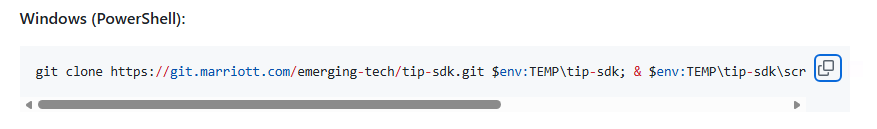
\includegraphics[width=0.95\textwidth]{ps-vdi-10-clone-cmd.png}
\caption{The one-liner from the README. Copy and paste into
PowerShell.}
\end{figure}

\begin{lstlisting}[style=powershell]
git clone https://gitea.poyner.ai/sean/liteforge.git $env:TEMP\liteforge; & $env:TEMP\liteforge\scripts\install.ps1; Remove-Item -Recurse -Force $env:TEMP\liteforge
\end{lstlisting}

\begin{figure}[H]
\centering
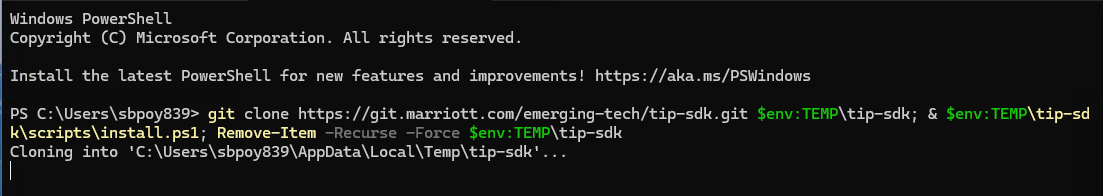
\includegraphics[width=0.95\textwidth]{ps-vdi-11-clone-start.png}
\caption{\texttt{git clone} starts. You may be prompted in your browser
to complete GitHub Enterprise authentication.}
\end{figure}

The installer detects your platform, copies the corporate CA bundle to
\texttt{\%USERPROFILE\%\textbackslash.forge\textbackslash certs}, and offers
to add the certs to the Windows certificate store:

\begin{figure}[H]
\centering
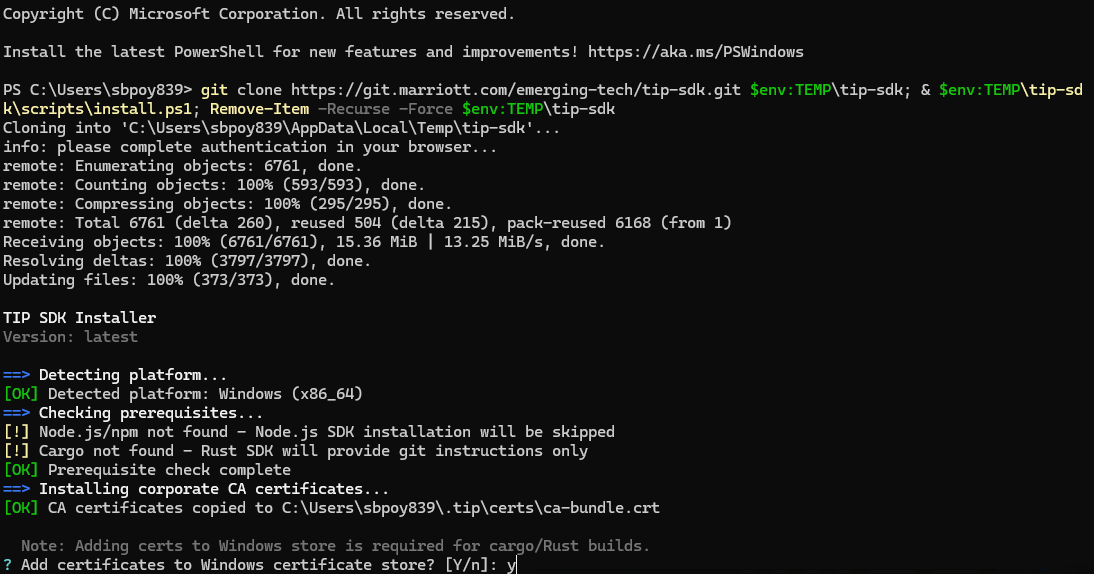
\includegraphics[width=0.95\textwidth]{ps-vdi-12-installer-start.png}
\caption{Platform detection, prerequisite checks, and CA certificate
copy. Answer \textbf{y} to add certificates to the Windows store.}
\end{figure}

\begin{figure}[H]
\centering
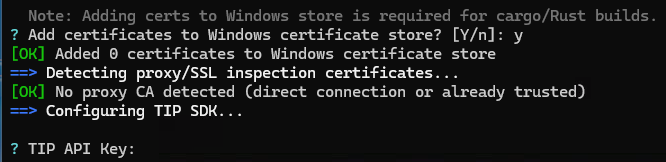
\includegraphics[width=0.85\textwidth]{ps-vdi-13-cert-config.png}
\caption{Proxy / SSL inspection certificates are detected automatically
on managed VDIs.}
\end{figure}

\newpage
% ============================================================================
\section{Step 6: Configure LiteForge}
% ============================================================================

The installer prompts for your LiteForge configuration. Press \textbf{Enter} on
any prompt to accept the default shown in brackets.

\begin{table}[H]
\centering
\begin{tabularx}{0.9\textwidth}{@{}>{\bfseries}l X@{}}
\toprule
Prompt & What to enter \\
\midrule
LiteForge API Key & Your personal API key (required, hidden as you type) \\
LiteForge Base URL & Press Enter for default \\
Default Model & Press Enter for \texttt{anthropic.claude-haiku-4-5-20251001-v1:0} \\
Knowledge Service URL & Press Enter to skip \\
Temporal Endpoint & Press Enter to skip \\
\bottomrule
\end{tabularx}
\caption{Installer configuration prompts and recommended values.}
\end{table}

\begin{figure}[H]
\centering
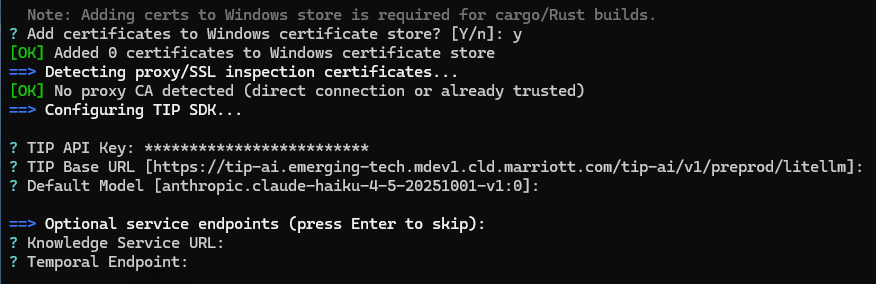
\includegraphics[width=0.95\textwidth]{ps-vdi-14-config-prompts.png}
\caption{Configuration prompts for API key, base URL, default model,
and optional service endpoints.}
\end{figure}

After credentials are validated, choose which components to install.
The list is conditional: each SDK only appears if the corresponding
toolchain is on your PATH (Python for \texttt{liteforge-py}, Node/npm
for \texttt{liteforge-js}, Rust/cargo for \texttt{liteforge}). If you did
not install Node in Step~4, the \texttt{liteforge-js} prompt will not
appear at all --- install Node and re-run the installer to add it
later. The same applies to Python and Rust.

\begin{figure}[H]
\centering
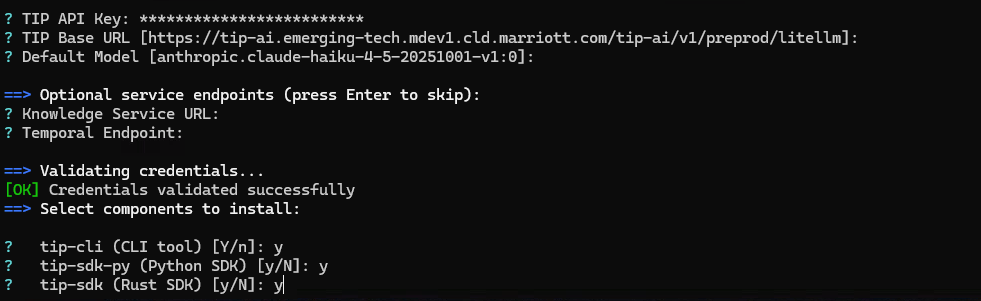
\includegraphics[width=0.95\textwidth]{ps-vdi-15-component-select.png}
\caption{Component selection. The Node.js SDK row will appear here as
\texttt{liteforge-js (Node.js SDK) [y/N]} when \texttt{npm} is on the
PATH; otherwise it is silently skipped.}
\end{figure}

\subsection{What the installer does}

The installer prefers pre-built artifacts shipped in the repo's
\texttt{bin/} directory. If those are missing, it falls back to building
from source with \texttt{cargo} and \texttt{maturin}, then to downloading
from GitHub releases. On a VDI where binary downloads are corrupted by
the proxy, the pre-built path is by far the most reliable.

\begin{figure}[H]
\centering
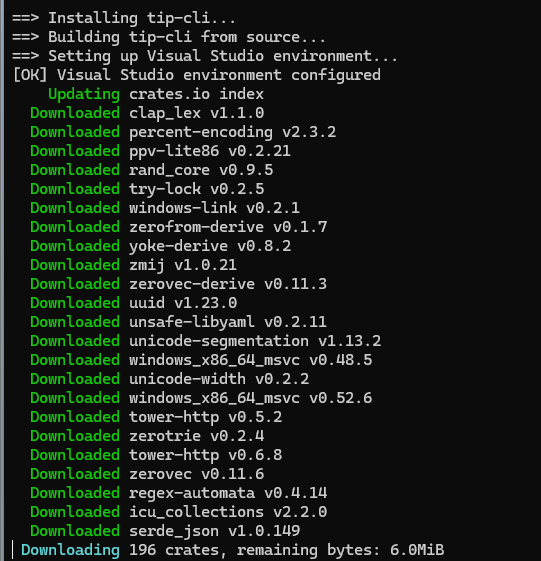
\includegraphics[width=0.85\textwidth]{ps-vdi-16-building-cli.png}
\caption{Fallback path: when the pre-built binary is unavailable, the
installer builds \texttt{forge-cli} from source. Requires Rust and the
Visual C++ Build Tools from Steps 1--2.}
\end{figure}

\newpage
% ============================================================================
\section{Step 7: Verify Installation}
% ============================================================================

The installer ends with a summary and writes
\texttt{\%USERPROFILE\%\textbackslash.forge\textbackslash bin} to your user
PATH:

\begin{figure}[H]
\centering
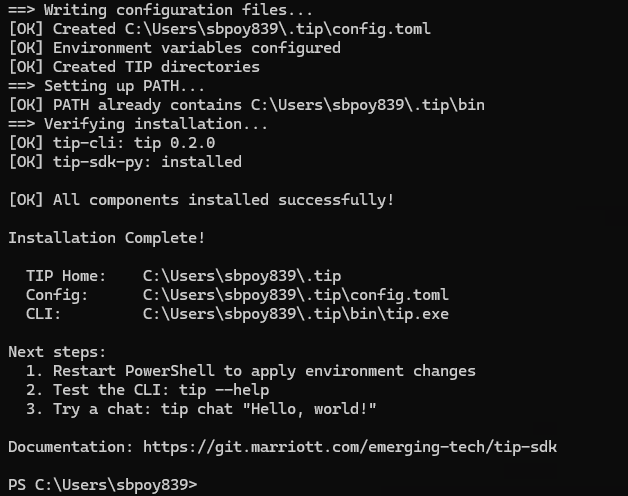
\includegraphics[width=0.85\textwidth]{ps-vdi-17-install-complete.png}
\caption{Installation complete. Both \texttt{forge-cli} and
\texttt{liteforge-py} report \texttt{[OK]}.}
\end{figure}

\textbf{Close and re-open PowerShell} so the PATH change takes effect,
then run:

\begin{lstlisting}[style=powershell]
forge --help
\end{lstlisting}

\begin{figure}[H]
\centering
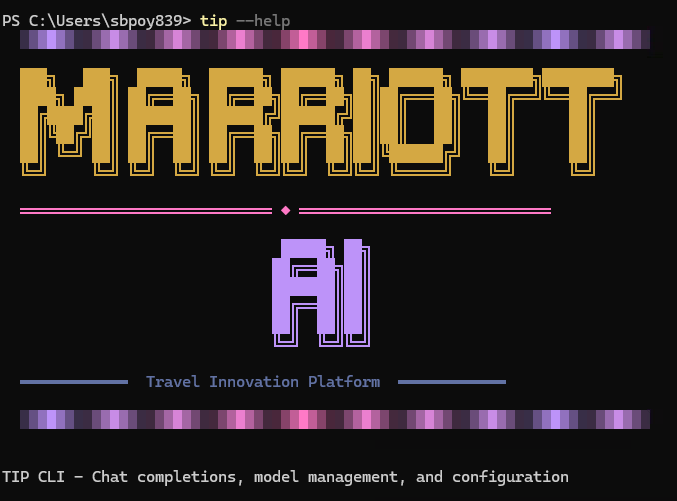
\includegraphics[width=0.95\textwidth]{ps-vdi-18-forge-help.png}
\caption{The \texttt{forge --help} output with the Forge banner ---
the CLI is on your PATH and ready.}
\end{figure}

\begin{tcolorbox}[tipbox={First chat}]
Try a chat completion to confirm everything works end-to-end:
\begin{lstlisting}[style=powershell]
forge chat -s "You are a space pirate that loots other ships by hacking them" -i
\end{lstlisting}
The \texttt{-s} flag sets a system prompt and \texttt{-i} drops you into
an interactive REPL.
\end{tcolorbox}

\begin{figure}[H]
\centering
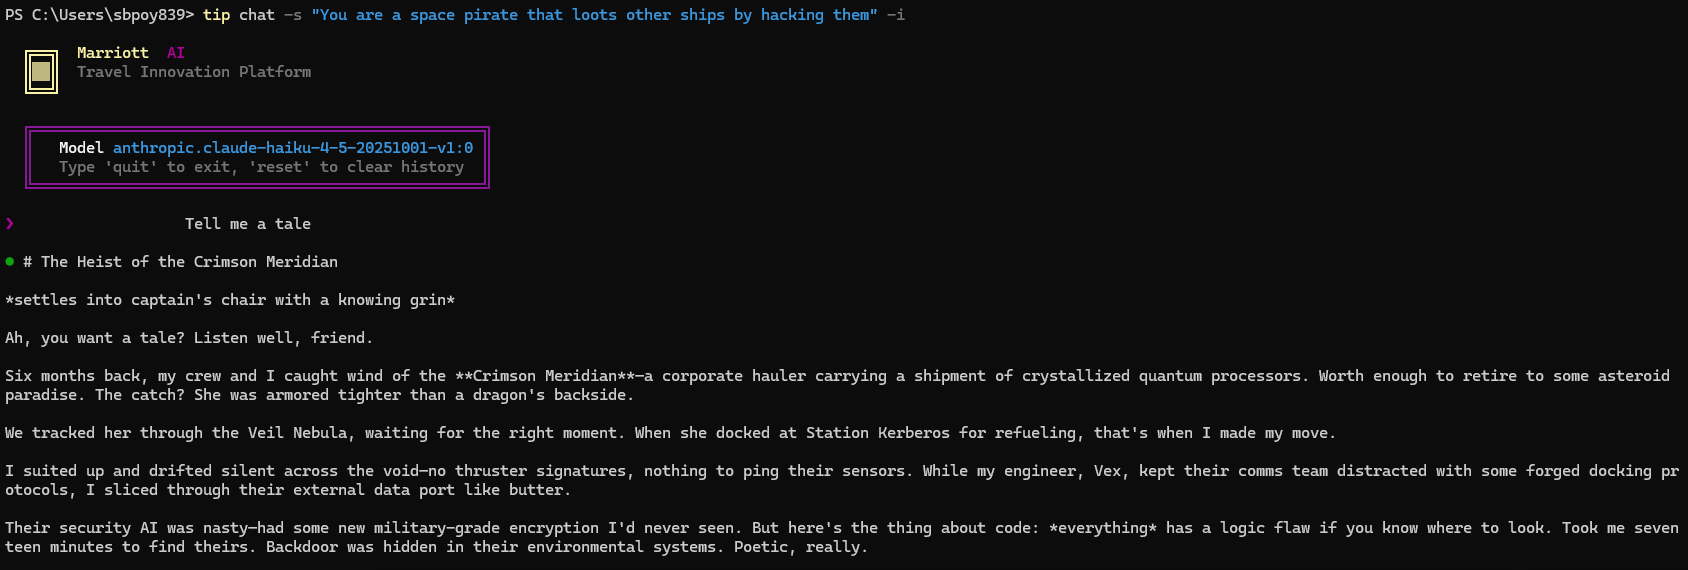
\includegraphics[width=0.95\textwidth]{ps-vdi-19-forge-chat.png}
\caption{Interactive chat with a custom system prompt --- streamed from
the LiteForge gateway through the configured default model.}
\end{figure}

\newpage
% ============================================================================
\section{Troubleshooting}
% ============================================================================

\subsection{``LNK1181: cannot open input file `kernel32.lib'\,''}

\begin{tcolorbox}[warnbox={Error}]
\texttt{LINK : fatal error LNK1181: cannot open input file 'kernel32.lib'}
\end{tcolorbox}

\textbf{Cause:} The MSVC linker is installed but the Windows SDK is not.
This happens when the silent Build Tools install ran but skipped the SDK
component.

\textbf{Fix:} Re-run Step~2 with the GUI installer and explicitly check
the Windows 11 (or 10) SDK box.

\subsection{``End of Central Directory record could not be found''}

\begin{tcolorbox}[warnbox={Error}]
\texttt{New-Object : Exception calling ".ctor" with "3" argument(s):
"End of Central Directory record could not be found."}
\end{tcolorbox}

\textbf{Cause:} The pre-built ZIP downloaded from
\texttt{gitea.poyner.ai} was corrupted in transit by the corporate
proxy / DLP / SSL inspection layer. This is common on enterprise VDIs.

\textbf{Fix:} The current installer prefers the binary checked into the
repo at \texttt{bin/forge-x86\_64-pc-windows-gnu.exe} \emph{before} trying
the GitHub release download, so a fresh \texttt{git clone} should hit
the working path automatically. If you have an older clone, pull the
latest \texttt{main}.

\subsection{Build from source fails with download timeouts}

\begin{tcolorbox}[warnbox={Error}]
\texttt{warning: spurious network error: Timeout was reached (download of
`windows\_x86\_64\_gnullvm v0.52.6` failed to transfer more than 10 bytes
in 30s)}
\end{tcolorbox}

\textbf{Cause:} The VDI proxy is throttling or blocking some
\texttt{crates.io} downloads.

\textbf{Fix:} The installer ships a pre-built Python wheel
(\texttt{bin/forge\_sdk-*-cp312-cp312-win\_amd64.whl}) that bypasses
\texttt{cargo build} entirely. Make sure you are on Python 3.12 so the
wheel matches.

\subsection{Garbled installer output}

If you see prompts run together or output appearing on the wrong line in
older PowerShell hosts, ensure you are on the latest \texttt{install.ps1}
--- the script was updated to use \texttt{Read-Host -Prompt} and
\texttt{Write-Output} (instead of split \texttt{Write-Host -NoNewline}
calls) for VDI terminal compatibility.

\subsection{Microsoft Store opens when running \texttt{python}}

\textbf{Cause:} The Windows App Execution Alias for \texttt{python.exe}
points to the Microsoft Store stub.

\textbf{Fix:} Either install Python via \texttt{python.org} (Step~3,
Option A) which writes a real interpreter to your user profile, or
disable the alias:
\textit{Settings $\to$ Apps $\to$ Advanced app settings $\to$ App
execution aliases $\to$ python.exe $\to$ off}.

\subsection{Certificate / TLS errors}

\textbf{Fix:} Re-run the installer or manually verify the bundle:

\begin{lstlisting}[style=powershell]
Test-Path $env:USERPROFILE\.forge\certs\ca-bundle.crt
[Environment]::GetEnvironmentVariable("SSL_CERT_FILE","User")
\end{lstlisting}

If \texttt{cargo} fails revocation checks against a corporate-signed
proxy CA, set:

\begin{lstlisting}[style=powershell]
[Environment]::SetEnvironmentVariable("CARGO_HTTP_CHECK_REVOKE","false","User")
\end{lstlisting}

\newpage
% ============================================================================
\section{Quick Reference}
% ============================================================================

\begin{table}[H]
\centering
\renewcommand{\arraystretch}{1.3}
\begin{tabularx}{\textwidth}{@{}>{\ttfamily\small}l X@{}}
\toprule
\textnormal{\textbf{Command}} & \textbf{Description} \\
\midrule
forge chat "..." & Chat with an LLM \\
forge chat -i & Interactive REPL mode \\
forge chat --stream "..." & Streaming response \\
forge models & List available models \\
forge config show & Display all settings \\
forge config set api-key KEY & Set API key \\
forge claude & Launch Claude Code with LiteForge config \\
forge agents & List available agents \\
forge tools & List agent tools \\
forge embed "text" & Generate embeddings \\
forge chunk "text" & Split text into chunks \\
forge guardrails "text" & Check for PII / prompt injection \\
forge serve & Start multi-port agent server \\
forge adk init NAME & Scaffold an agent project \\
forge adk dev & Hot-reload dev server \\
forge adk build & Build container image \\
forge usage & View API usage reports \\
\bottomrule
\end{tabularx}
\caption{Forge CLI command quick reference.}
\end{table}

\begin{tcolorbox}[infobox={Configuration Locations (Windows)}]
\begin{tabularx}{\textwidth}{@{}>{\ttfamily\small}l X@{}}
\%USERPROFILE\%\textbackslash.forge\textbackslash config.toml & Main configuration (API key, base URL, model) \\
\%USERPROFILE\%\textbackslash.forge\textbackslash certs\textbackslash ca-bundle.crt & Corporate CA certificate bundle \\
\%USERPROFILE\%\textbackslash.forge\textbackslash bin\textbackslash forge.exe & CLI binary location \\
HKCU Environment & LiteForge\_API\_KEY, LiteForge\_BASE\_URL, LiteForge\_DEFAULT\_MODEL, SSL\_CERT\_FILE \\
\end{tabularx}
\end{tcolorbox}

\vfill

\begin{center}
\small\color{forgegray}
\rule{0.6\textwidth}{0.4pt}\\[6pt]
LiteForge v0.2.0 -- LiteForge\\
\textcolor{alertred}{\textit{Proprietary and Confidential}}
\end{center}

\end{document}
